
\subsection{Answers}
\begin{table}[htb]%
\begin{center}%
\caption{Q18: Which MPI thread support are you using?}%
\label{tab:Q18-ans}%
\begin{tabular}{l|l|r}%
\hline%
Choice & Abbrv. & \# Answers \\%
\hline%
MPI\_THREAD\_SINGLE & SINGLE & 238 (28.7\%) \\%
MPI\_THREAD\_FUNNELED & FUNNELED & 145 (17.5\%) \\%
MPI\_THREAD\_SERIALIZED & SERIALIZED & 99 (11.9\%) \\%
MPI\_THREAD\_MULTIPLE & MULTIPLE & 261 (31.4\%) \\%
I have never called MPI\_INIT\_THREAD & never used & 267 (32.2\%) \\%
I do not know or I do not care. & do not know/care & 168 (20.2\%) \\%
\hline%
\multicolumn{2}{c}{total} & 1178 (830)\\%
\hline%
\end{tabular}%
\end{center}%
\end{table}%


\begin{figure}[htb]
\begin{center}
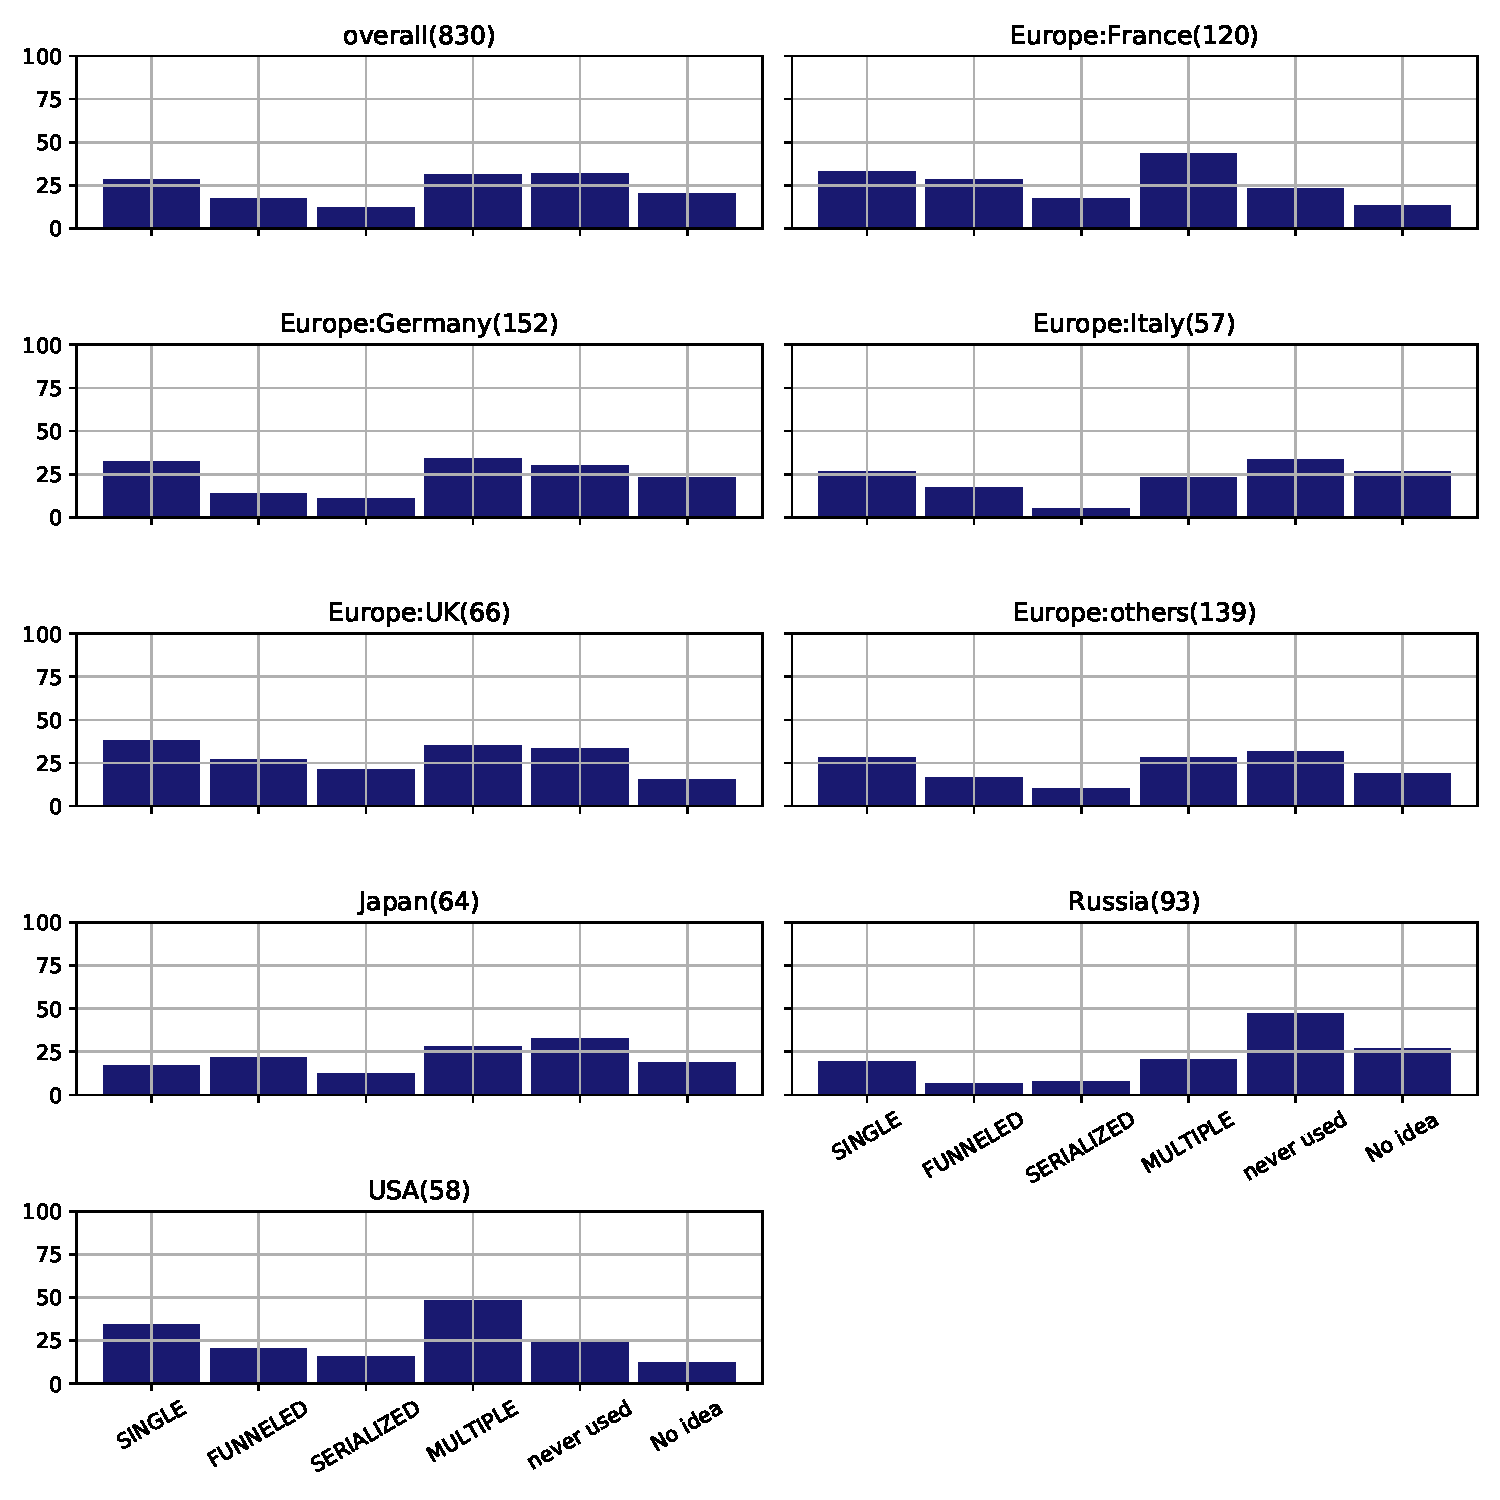
\includegraphics[width=10cm]{../pdfs/Q18.pdf}
\caption{Simple analysis: Q18}
\label{fig:Q18}
\end{center}
\end{figure}

The support of multi-threading in MPI is done in different ways (MPI\_THREAD\_SINGLE
MPI\_THREAD\_FUNNELED, MPI\_THREAD\_SERIALIZED, MPI\_THREAD\_MULTIPLE, in order of
decreasing semantic restriction). If used the most used option (42\%) are either
MPI\_THREAD\_SINGLE or MPI\_THREAD\_MULTIPLE which are the at the two and of the
spectrum in terms of thread support: most users either want a full support or a
limited support. Moreover, almost 40\% of the respondent have no usage of thread
support in their program. Region-wise, we see that in the USA, thread support is more used
than in other region and the most used option is MPI\_THREAD\_MULTIPLE which is
the least restrictive option. 

This is a multiple-answer question.  In Table~\ref{tab:Q18-mans}, the
number of participants who answered ``I have never called
MPI\_INIT\_THREAD'' and ``I do not know or I do not care'' dominates
close to 50\%  (note that the numbers of answers are shown
in Table~\ref{tab:Q18-ans}). In the rest of the half, the
number of specifying one of the thread level and the number of
specifying two or more of them are comparable. 


\clearpage%
{\footnotesize\begin{landscape}%
\begin{longtable}[htb]{r|c|c|c|c|c|c|c|c|c|c}%
\caption{Q18: Which MPI thread support are you using?}%
\label{tab:Q18-mans} \\%
\hline%
Multi-Answer & overall & FR & GR & IT & UK & eu & JP & RU & US & others \\
 \hline%
\endfirsthead%
\multicolumn{11}{r}{(continued from the previous page)}\\%
\hline%
Multi-Answer & overall & FR & GR & IT & UK & eu & JP & RU & US & others \\
 \hline%
\endhead%
\hline%
(total) & 830 & 120 & 152 & 57 & 66 & 139 & 64 & 93 & 58 & 81 \\%
\hline%
\multicolumn{11}{r}{(continue to the next page)}\\%
\endfoot%
\hline%
(total) & 830 & 120 & 152 & 57 & 66 & 139 & 64 & 93 & 58 & 81 \\%
\hline%
\endlastfoot%
\hline%
{never used} & 234 & 24 & 40 & 15 & 20 & 40 & 19 & 39 & 14 & 23 \\%
{No idea} & 143 & 14 & 29 & 13 & 8 & 25 & 11 & 20 & 5 & 18 \\%
{MULTIPLE} & 97 & 18 & 19 & 7 & 7 & 15 & 9 & 5 & 8 & 9 \\%
{SINGLE, MULTIPLE} & 70 & 11 & 17 & 3 & 4 & 13 & 2 & 9 & 6 & 5 \\%
{SINGLE} & 59 & 7 & 12 & 6 & 5 & 11 & 1 & 2 & 5 & 10 \\%
{FUNNELED} & 36 & 5 & 4 & 5 & 1 & 11 & 4 & 3 & 1 & 2 \\%
{SINGLE, FUNNELED, SERIALIZED, MULTIPLE} & 34 & 9 & 9 & 2 & 8 & 1 & 1 & 0 & 3 & 1 \\%
{SINGLE, FUNNELED} & 28 & 8 & 7 & 1 & 3 & 3 & 3 & 1 & 0 & 2 \\%
{never used, No idea} & 23 & 2 & 6 & 2 & 2 & 1 & 1 & 5 & 1 & 3 \\%
{SERIALIZED} & 23 & 5 & 1 & 0 & 1 & 3 & 4 & 2 & 4 & 3 \\%
{FUNNELED, MULTIPLE} & 18 & 7 & 0 & 0 & 0 & 1 & 4 & 0 & 5 & 1 \\%
{SINGLE, FUNNELED, MULTIPLE} & 12 & 1 & 1 & 0 & 2 & 2 & 1 & 2 & 3 & 0 \\%
{SINGLE, SERIALIZED, MULTIPLE} & 10 & 1 & 2 & 0 & 0 & 3 & 0 & 2 & 2 & 0 \\%
{SERIALIZED, MULTIPLE} & 10 & 1 & 4 & 0 & 1 & 2 & 1 & 1 & 0 & 0 \\%
{SINGLE, FUNNELED, SERIALIZED} & 9 & 0 & 0 & 1 & 3 & 3 & 1 & 0 & 0 & 1 \\%
{SINGLE, SERIALIZED} & 7 & 1 & 1 & 0 & 0 & 1 & 1 & 2 & 0 & 1 \\%
{FUNNELED, SERIALIZED, MULTIPLE} & 5 & 3 & 0 & 0 & 1 & 1 & 0 & 0 & 0 & 0 \\%
{SINGLE, never used} & 5 & 1 & 0 & 1 & 0 & 1 & 1 & 0 & 0 & 1 \\%
{SINGLE, MULTIPLE, never used} & 2 & 1 & 0 & 0 & 0 & 1 & 0 & 0 & 0 & 0 \\%
{SINGLE, FUNNELED, MULTIPLE, never used} & 1 & 0 & 0 & 1 & 0 & 0 & 0 & 0 & 0 & 0 \\%
{FUNNELED, never used} & 1 & 0 & 0 & 0 & 0 & 1 & 0 & 0 & 0 & 0 \\%
{MULTIPLE, never used, No idea} & 1 & 0 & 0 & 0 & 0 & 0 & 0 & 0 & 0 & 1 \\%
{SINGLE, MULTIPLE, No idea} & 1 & 0 & 0 & 0 & 0 & 0 & 0 & 0 & 1 & 0 \\%
{FUNNELED, SERIALIZED} & 1 & 1 & 0 & 0 & 0 & 0 & 0 & 0 & 0 & 0 \\%
\hline%
\end{longtable}%
\end{landscape}}%
\clearpage%

